% Chapter 3

\chapter{Analysis} % Main chapter title
\label{chap:Chapter3} % For referencing the chapter elsewhere, use \ref{chap:Chapter3} 

In this chapter it will be presented a bussiness value analysis of the project and the reasoning behind it. 

\section{Engineering Requirements}

This section \dots the process of analysing the functional and non-functional requirements of this project.

\subsection{Functional Requirements}

\dots

\subsection{Non-functional Requirements}

\dots

\section{Value Analysis}

In order to develop a new product there is a need for a value analysing in order to properly assess the relation between cost and value.
The analysis presented in the following subsections will follow the New Concept Development Model (NCD) (\cite{koen_2001}) approach.

\subsection{New Concept Development Model}

\dots

The model as defined by Koen, is composed by five key stages:

\begin{itemize}
    \item Opportunity identification - The opportunity was identified by a member of the deaf community.
    He claimed that there were no solution to help the process of explaning a given concept using sign language.
    The lexicon of \gls{PSL} is quite small so most words don't have a direct translation, therefore it is required to use the available gestures to explain them.

    \item Opportunity analysis - When analysing the market, the only tools that have some similarities are the sign language dictionaries but they have some limitation that make it impossible to be a viable solution.
    One of this limitations is that a translation to be added requires that a person is recorded performing the signs required to reproduce the word or expression.
    Another limitation of those dictionaries is the lack of translations for word from the scientific domain.

    \item Idea creation - In this stage, \dots ideas for a solution that targets the identified opportunity and is a better fit over the other alternatives analysed.
    One idea is that the solution to be developed makes the process of explaning a concept automatic.
    For this, the explanation can be found somewhere online and it is possible to obtain it using Information Retrival, Information Extraction and Text Mining techniques.
    To make the obtained explanation viable to be presented to a member of the deaf community it would be better to translate it to \gls{PSL}.
    For this, there is another GILT project that is already capable of performing this translation and the \gls{API} behind it can be used in this solution.

    \item Idea selection - In this stage, the goal was to take all the possible ideas an approaches in a single one that fulfills the necessary requirements.
    The resulting idea is to develop an automatic interpretation system having the needs of the deaf community in mind.
    This system will use Information Retrival, Information Extraction and Text Mining to generate the explanation of a given word or expression.
    It will also translate said explanation to \gls{PSL}.

    \item Concept definition - After having the idea selected the next step is to define the objectives needed to achieve it.
    The goals of this project are to develop an \gls{API} capable of generating the explanation of a given concept and a web application that will use this, and another \gls{API} to help the deaf community in the process of concept explanation. 

\end{itemize}

\subsection{Value}

Value for customer, Perceived Value, Benefits, Sacrifices

The benefit that was identified is \dots helping in the process of explaning a concept using sign language.

The identified sacrifices are the need for a device that is able to connect to the internet.

\dots

\subsection{Value Proposition}

A value proposition is 

\subsection{CANVAS model}

\dots

\begin{figure}[H]
\centering
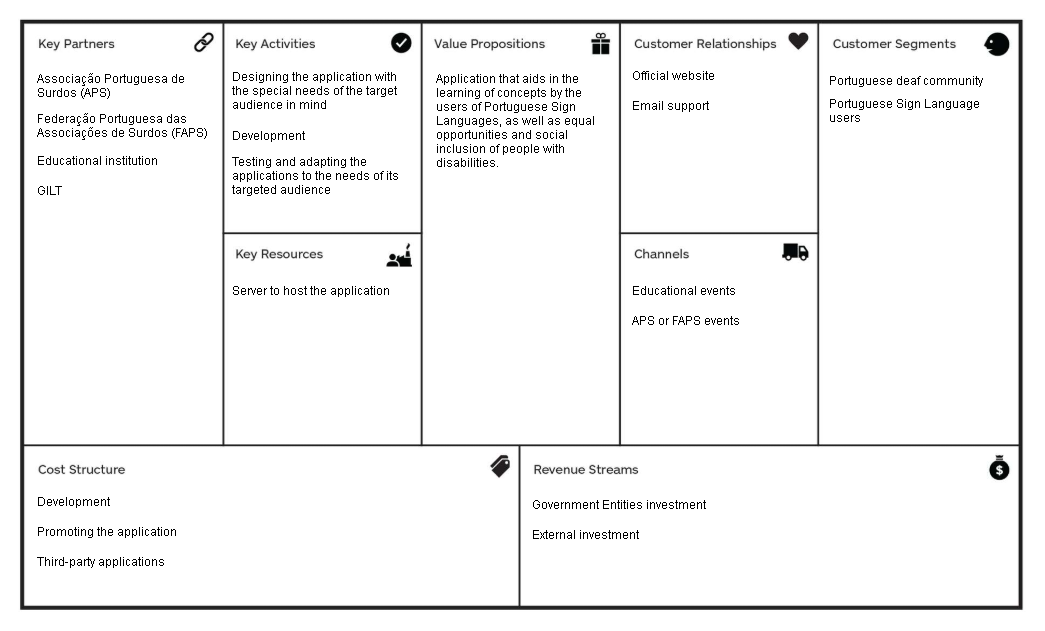
\includegraphics[width=\textwidth,keepaspectratio]{ch2/assets/CANVAS.png}
\caption[CANVAS]{CANVAS Model}
\label{fig:CANVAS}
\end{figure}

\subsection{AHP}

\dots

\begin{figure}[H]
\centering
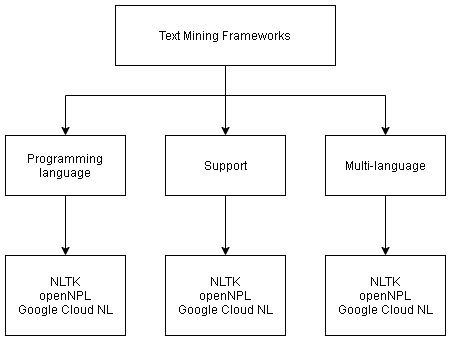
\includegraphics[scale=0.5]{ch2/assets/AHP.png}
\caption[AHP Hierarchy Division]{AHP Hierarchy Division}
\label{fig:AHP}
\end{figure}

As observed in the Figure~\ref{fig:AHP}, the items of the first layer, corresponding to the primary objectives, had the following criteria behind their selection:

\begin{itemize}
    \item Programming language - The language to be used for developing the solution \gls{API}.
    \item Support - The number of reliable sources of information, the quality of the documentation and an active community.
    \item Multi-language - The compatibility of processing texts and performing tasks using different languages. 
\end{itemize}


\begin{table}[H]
\caption{Fundamental scale \autocite{saaty_1987}.}
\label{tab:scale}
\centering
\begin{tabular}{|m{4cm}|m{4cm}|m{4cm}|}
\hline
\tabhead{Intensity of importance on an absolute scale} & \tabhead{Definition} & \tabhead{Explanation} \\
\hline
1 & Equal importance & Two activities contribute equally to the objective\\
\hline
3 & Moderate importance of one over another & Experience and judgment strongly favor one activity over another\\
\hline
5 & Essential or strong importance & Experience and judgment strongly favor one activity over another\\
\hline
7 & Very strong importance & An activity is strongly favored and its dominance demonstrated in practice\\
\hline
9 & Extreme importance & The evidence favoring one activity over another is of the highest possible order of affirmation \\
\hline
2,4,6,8 & Intermediate values between two adjacent judgments & When compromise is needed \\
\hline
\end{tabular}
\end{table}

